%!TEX root = Thesis_main.tex

\chapter{Kinematic Model of the Mobile Manipulator}
\label{chapter2}
\section{Mobile Robot Model}
\subsubsection{Holonomic and Nonholonomic constraints}
Constraints which reduce the dimensions of the accessible configuration space of a system of rigid bodies, i.e. acting on the generalized coordinates $x$ that describe the system, are said to be \textit{holonomic} or integrable. 
Holonomic constraints are expressed in the form:
\begin{equation}
h\left( x\right) =0
\end{equation}
All constraints which instead are nonintegrable are said to be \textit{nonholonomic}, so also inequality constraints on the configuration space. In particular, constraints on the generalized velocities of the system of rigid bodies but not on its configuration are nonholonomic.\\
Nonholonomic constraints reduce the mobility of the mechanical system in a completely different way with respect to holonomic constraints. The fact that the constraint is nonintegrable means that there is no loss of accessibility to the entire configuration space for the system. In other words, while the subspace of the generalized velocities is reduced due to the constraint, the number of generalized coordinates cannot be reduced.
Nonholonomic constraints are expressed in the form:
\begin{equation}
h( x,\dot{x}) =0
\end{equation}
Kinematic constraints both holonomic or nonholonomic are usually written in the Pfaffian form, i.e. linearly with respect to the generalized velocities.
\begin{equation}
a_i^T \left( x \right)\dot{x} =0 \qquad i=1,...,k<n 
\end{equation}
or in a compact form:
\begin{equation} 
A^T \left( x \right)\dot{x} =0  
\end{equation}
Assuming now to have $k$ nonholonomic constraint equations for a $n$ dimensional system, this implies that the admissible generalized velocities $\dot{x}$ of the system in any of its configuration $x$ necessarily belong to a $(n-k)$-dimensional space. Specifically, expressing the constraint equations in Pfaffian form, the generalized velocities should belong to the null space of matrix $A^T$.\\
Thus, it can be written as
\begin{equation} \label{G}
\dot{x}=\sum_{j=1}^{m} g_j(x)u_j=G(x)u \qquad m=n-k
\end{equation}
where $x\in \mathbb{R}^n $ is the vector of the generalized coordinates describing the system (state vector), $u= \left[
\begin{matrix}
u_1 &  \cdots & u_m
\end{matrix}
\right]^T\in\mathbb{R}^m $ is the vector of input velocities and $\left\lbrace  g_1(x) \cdots g_m(x) \right\rbrace $ is a basis of the null space of $A^T$.\\ 
Talking about mobile robots, wheels are by far the most common mechanism to achieve locomotion. Any wheeled vehicle is subject to kinematic pure rolling constraints that reduce in general its local mobility, while leaving intact the possibility of reaching arbitrary configurations by appropriate manoeuvres. The pure rolling constraint is nonholonomic, because it implies no loss of accessibility in the configuration space of the vehicle.\\
The kinematics of a wheeled mobile robot subjected to pure rolling constraints changes depending on how locomotion is achieved. Mainly there are two types of wheeled mobile robot models: unicycle like robots and bicycle like ones. We will focus on the first one.
\subsubsection{Unicycle Model}
\begin{figure}[h!]
	\centering
	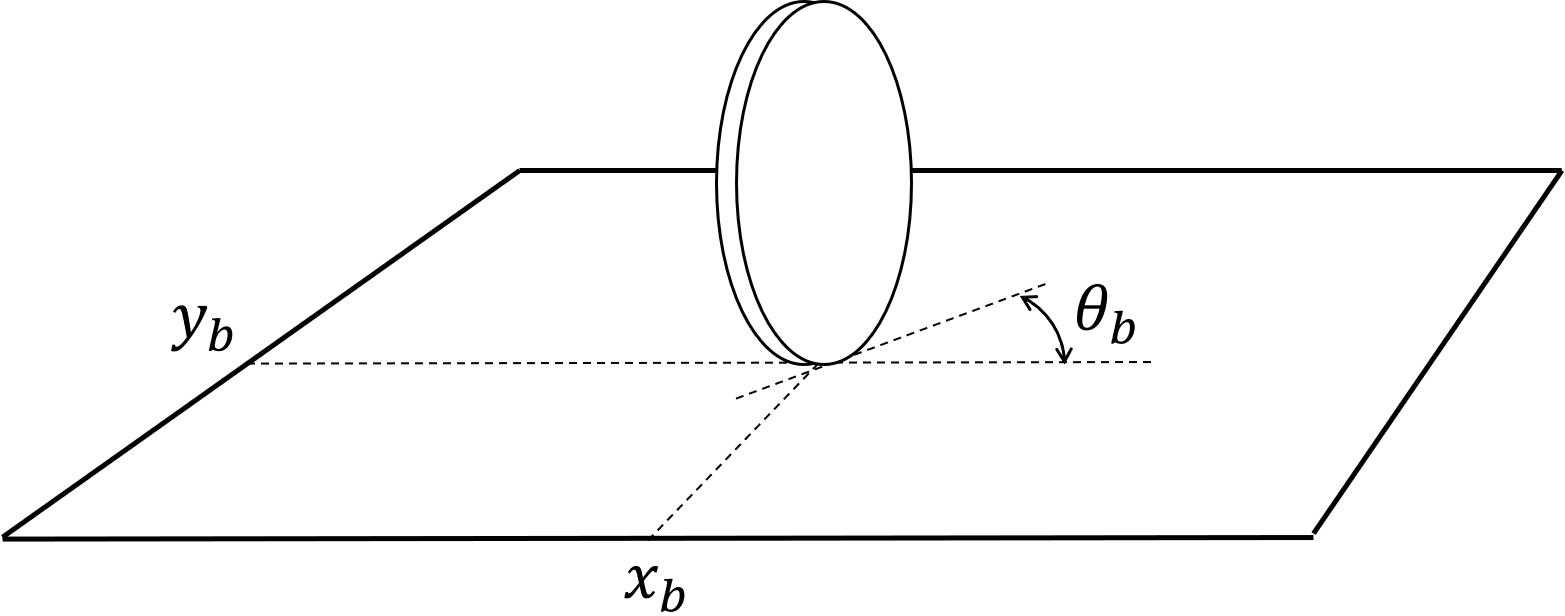
\includegraphics[scale=0.4]{unicyclemodel}
	\caption{Unicycle model}
	\label{fig:unicyclemodel}
\end{figure}
A unicycle is a vehicle whose configuration is completely described by the configuration vector $x = \left[\begin{matrix}x_b&y_b&\theta_b\end{matrix}\right]^T$, where $x_b$ and $y_b$ are the Cartesian coordinates of the contact point of the wheel with the ground and $\theta_b$ is the orientation of the wheel with respect to the axis of the abscissas, as showed in Figure \ref{fig:unicyclemodel}. \\
The pure rolling constraint for the unicycle is simply expressed as:
\begin{equation} \label{At}
\dot{x}_b\sin\theta_b-\dot{y}_b\cos\theta_b=\left[
\begin{matrix}
\sin\theta_b & \cos\theta_b & 0
\end{matrix}
\right] \dot{x}= A^T \left( x \right)\dot{x} =0  
\end{equation}
This equation expresses that the velocity of the contact point (or of the wheel centre) is zero in the direction orthogonal to the sagittal plane of the disk.\\
Hence the unicycle is a 3-dimensional system subject to one nonholonomic constraint, so the dimension of the basis of the null space of $A^T$ is 2. Choosing:
\begin{equation} \label{Gmatrix_def}
G(x)=\left[
\begin{matrix}
g_1 (x) & g_2 (x)
\end{matrix}
\right] =  \left[
\begin{matrix}
\cos\theta_b & 0 \\
\sin\theta_b & 0 \\
0 & 1 
\end{matrix}
\right] 
\end{equation}
All the admissible generalized velocities of the unicycle at $x$ are a combination of $g_1 (x)$ and $g_2 (x)$.
\begin{equation} 
\dot{x}=\left[
\begin{matrix}
\dot{x}_b \\ \dot{y}_b \\\dot{\theta}_b
\end{matrix}
\right] =  \left[
\begin{matrix}
\cos\theta_b \\ \sin\theta_b \\ 0 
\end{matrix}
\right]v + \left[
\begin{matrix}
0 \\ 0 \\ 1 
\end{matrix}
\right]\omega
\end{equation}
where $v$ and $\omega$ can be easily interepreted as the driving velocity, i.e. the velocity of the disk along its sagittal plane, and the steering velocity, i.e. the angular speed around its vertical axis.\\
A lot of mobile robots are kinematically equivalent to a unicycle, like differential drive robots, like the one in Figure \ref{fig:mobilebase}, skid steering robots or synchro drive vehicles.\\
In most of the unicycle-like mobile robots, $v$ and $\omega$ are the command input to the system, while the actual velocity input are $\omega_R$ and $\omega_L$, i.e. the right and left wheels angular speeds: 
\begin{equation}
v=\frac{r\left(\omega_R + \omega_L\right)}{2} \qquad \omega=\frac{r\left(\omega_R - \omega_L\right)}{d}
\end{equation}
\begin{equation}
\omega_R =\frac{1}{r}\left(v+\frac{d}{2}\omega\right) \qquad \omega_L=\frac{1}{r}\left(v-\frac{d}{2}\omega\right)
\end{equation}
where $r$ is the wheel radius and $d$ is the distance between the left and right wheels.
\begin{figure}[h!]
	\centering
	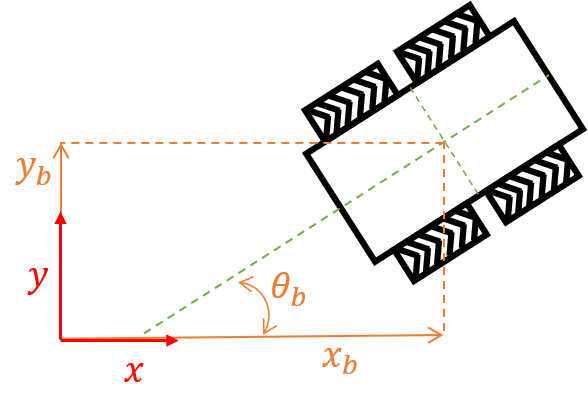
\includegraphics[scale=0.8]{mobilebase}
	\caption{Scheme of a Differential Drive Mobile Robot}
	\label{fig:mobilebase}
\end{figure}
\section{Manipulator Model}
A manipulator consists of a series of rigid links connected by joints. Mathematically it can be modeled as a kinematic chain where one end of the chain is constrained to a base, while an end effector is mounted to the other end. The end effector is used to manipulate objects in space, therefore it is the end effector position and orientation, \textit{pose}, that is often studied. \textit{Forward kinematics} describes the pose of the end effector as a function of the joint values:
\begin{equation}\label{forw_kin}
 	\xi=\left[\begin{matrix}p_{EE}\\\Phi_{EE}\end{matrix}\right]=f(x)
\end{equation} 
where $p_{EE}=\left[\begin{matrix}x_{EE}&y_{EE}&z_{EE}\end{matrix}\right]^T$ is the vector of the end effector Cartesian coordinates and $\Phi_{EE} =\left[\begin{matrix}\vartheta_{EE}&\varphi_{EE}&\psi_{EE}\end{matrix}\right]$ is the vector of the end effector orientation which can be expressed with different conventions like Azimut-Elevation-Rotation, or Roll-Pitch-Yaw. 
It is possible to express relation \eqref{forw_kin} in a compact form using the homogenous \textit{rototraslation matrix} $A_{ee}^{base}$ that describes the end effector reference frame with respect to the base global reference frame:
\begin{equation}\label{AAAA_man}
A_{ee}^{base}=A_1^{base}A_2^1A_3^2\cdots A_{ee}^{ee-1}
\end{equation}
where $A_i^{i-1}$ is the expression of the transformation from one joint frame to the following one through the use of Denavit-Hartemberg parameters \cite{DH}: $a\text{, }\alpha\text{, }d\text{, }\theta$ (defined as in Figure \ref{fig:DH}):
\begin{equation}
A_i^{i-1}=\left[
\begin{matrix}
\cos\theta & -\sin\theta\cos\alpha & \sin\theta\sin\alpha & a\cos\theta \\
\sin\theta & \cos\theta\cos\alpha & -\cos\theta\sin\alpha & a\sin\theta \\
0 & \sin\alpha & \cos\alpha & d \\
0 & 0 & 0 & 1
\end{matrix}
\right]
\end{equation}
This matrix is function only of the joint variables $\theta$ and $d$.

\begin{figure}[h!]
	\centering
	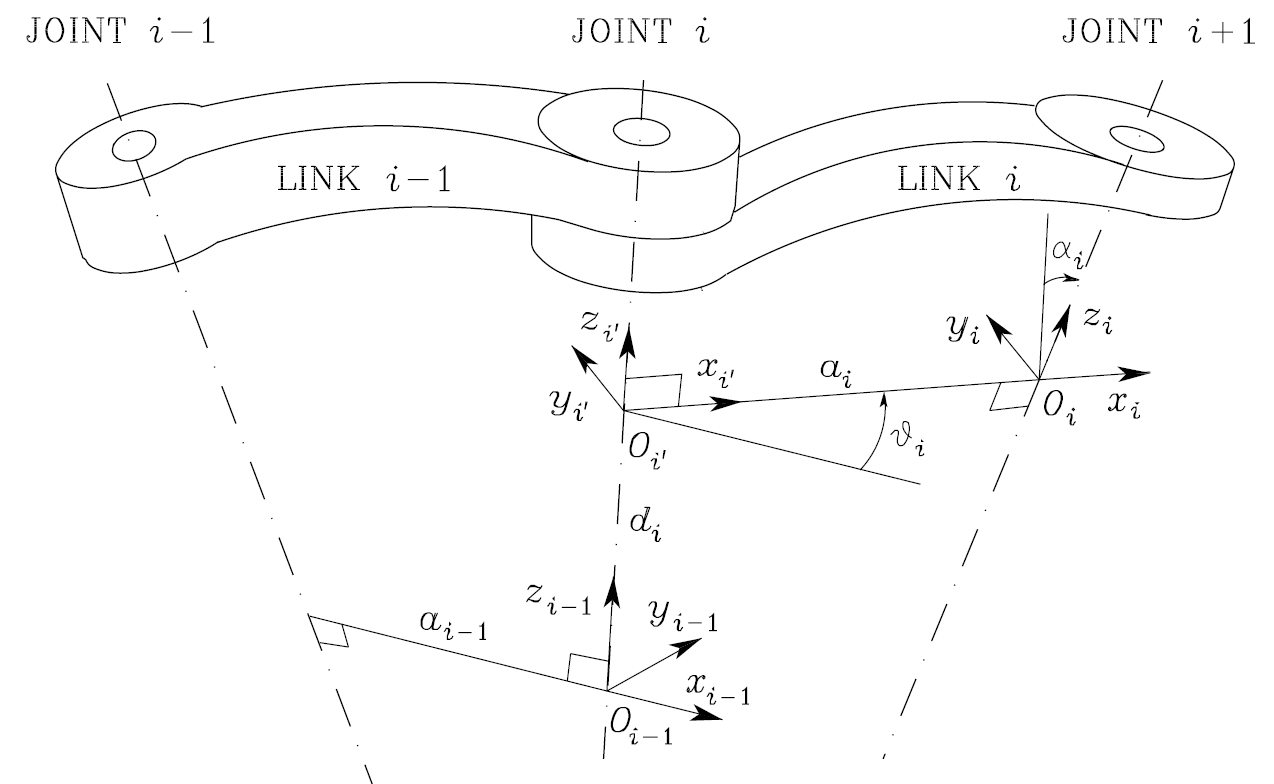
\includegraphics[scale=0.4]{denavithartenberg}
	\caption{Denavit-Hartenberg convention for Robot links}
	\label{fig:DH}
\end{figure}

The opposite problem is the definition of the \textit{inverse kinematics}, i.e. given the position and orientation of the end effector, the corresponding joint variables have to be found. The inverse kinematics problem is not easy to solve since it is often nonlinear and there can be infinite solutions as well as none.\\
An important concept which roboticists are still working on is \textit{kinematic redundancy}, i.e. the condition when the dimension of joint space is greater than the dimension of the operational space relative to the task to be achieved. For example, for a problem of end effector position and orientation regulation the task operational space is 6-dimensional, so a 7-Dof robotic system would be redundant.
When a system is kinematically redundant, direct kinematics is always possible to be defined, while inverse kinematics can have infinite solutions.
Solving the \textit{kinematic redundancy problem} means to define a criterion in order to be able to pick one among the infinite configurations which are a solution to the inverse kinematic problem.\\
This concept will be very important in the defintion of Mobile Manipulator control, since Mobile Manipulators are highly redundant systems.

\section{Mobile Manipulator Model}
\begin{figure}
\centering
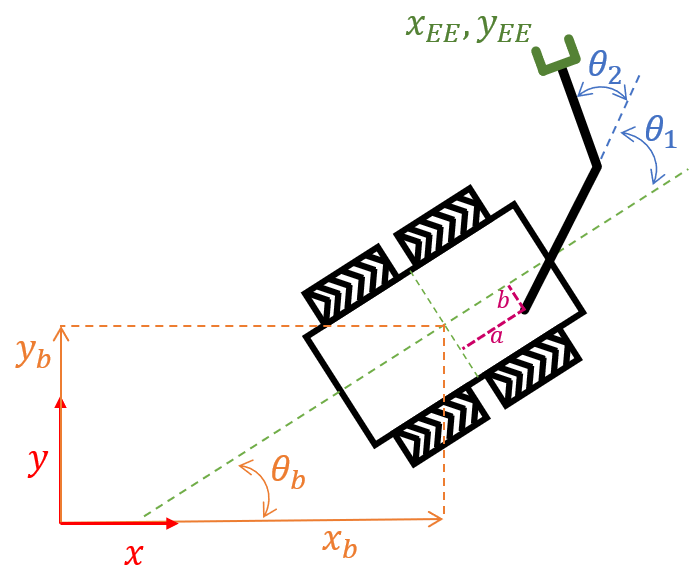
\includegraphics[scale=0.8]{MMkinematics}
\caption{A simple Mobile Manipulator composed by a mobile base and a 2-Dof robotic arm}
\label{fig:MMkinematics}
\end{figure}
Considering the general case of a Mobile Manipulator composed by a manipulator arm mounted on a mobile platform, its kinematic model set the location and orientation of the end effector as a function of both the arm and base generalized coordinates:
\begin{equation}\label{dirkinMM}
	\xi=\left[\begin{matrix}p_{EE}\\\Phi\end{matrix}\right]=f(x)=f\left(\left[\begin{matrix}x_{base}\\x_{arm} \end{matrix}\right]\right)
\end{equation}
where $x_{base}$ is the configuration vector of the mobile base and $x_{arm}$ is the vector of joint coordinates of the manipulator.
As an example, the forward kinematics for just the Cartesian coordinates of the end effector of the simplified system in Figure \ref{fig:MMkinematics} is
\begin{equation*}
\begin{split}
	x_{EE}&=x_b+a\cos\theta_b-b\sin\theta_b+l_1\cos\left(\theta_b+\theta_1\right)+l_2\cos\left(\theta_b+\theta_1+\theta_2\right)\\
	y_{EE}&=y_b+a\sin\theta_b-b\cos\theta_b+l_1\sin\left(\theta_b+\theta_1\right)+l_2\sin\left(\theta_b+\theta_1+\theta_2\right)
\end{split}
\end{equation*}
It is possible to express the function $f(x)$ of Equations \eqref{dirkinMM} as in \eqref{AAAA_man} premultiplying the rototranslation matrix $A_{base}^{global}$, relative to the mobile base motion, to the direct kinematics of the arm. In the case of the previous example:
\begin{equation}
	A_{base}^{global}=\left[\begin{matrix}
		\cos\theta_b&-\sin\theta_b&0&x_b+a\cos\theta_b-b\sin\theta_b\\
		\sin\theta_b&\cos\theta_b&0&y_b+a\sin\theta_b-b\cos\theta_b\\
		0&0&1&h_{base}\\
		0&0&0&1
	\end{matrix}\right]
\end{equation}
So the forward kinematics can be obtained consequently:
\begin{equation}\label{AAAA}
A_{ee}^{global}=A_{base}^{global}A_1^{base}A_2^1\cdots A_{ee}^{ee-1}
\end{equation}
\paragraph{Redundancy}
As we had briefly introduced before, a robot is kinematically redundant if the number of its degrees of freedom is greater than it is strictly necessary. In this sense redundancy is thus a concept relative to the given task. Mobile Manipulators are systems specifically built redundant in order to exploit the extra degrees of freedom to:
\begin{itemize}
	\item avoid collision with obstacles;
	\item avoid kinematic singularities;
	\item increase the manipulability of the system;
	\item move with lower joint velocities;
	\item etc.
\end{itemize}
A common way to deal with redundant systems is to move the problem at velocity level through the use of Jacobians, as we will see more in detail in the following chapters. 
\paragraph{Differential kinematics}Differentiating $f$, the differential forward kinematics of the Mobile Manipulator can be obtained:
\begin{equation}\label{eq:dotx_EE}
	\dot{\xi}=\mathcal{J}_b(x)\dot{x}_{base}+\mathcal{J}_a(x)\dot{x}_{arm}
\end{equation}
where the columns of $\mathcal{J}_a(x)={\partial f}/{\partial x_{arm}}(x)$ can be obtained as:
\begin{equation}
\mathit{j}_{P_j}^{(EE)}=
	\begin{cases}
	z_{j-1} & \text{for a \textit{prismatic} joint} \\
	z_{j-1}\times \left(p_{EE}-p_{j-1}\right) & \text{for a \textit{revolute} joint}	
	\end{cases}                                             
\end{equation}
\begin{equation}
	\mathit{j}_{O_j}^{(EE)}= 
	\begin{cases}
	0 & \text{for a \textit{prismatic} joint} \\
	z_{j-1} & \text{for a \textit{revolute} joint}	
	\end{cases} 
\end{equation}
and $\mathcal{J}_b(x)={\partial f}/{\partial x_{base}}(x)$ can be obtained at the same way considering $x_b$ and $y_b$ as prismatic joints and $\theta_b$ as a revolute joint of the compound system.\\
Considering $\mathcal{J}_b(x)$, the nonholonomic constraint of Equation \eqref{G} of the mobile platform should be taken into account:
\begin{equation}
	\mathcal{J}_b(x)\dot{x}_b=\mathcal{J}_b(x)G(x)v=\mathcal{J}_v(x)v
\end{equation}
Therefore is now possible to reformulate Equation \eqref{eq:dotx_EE} in a compact form to express the end effector traslational and rotational velocities as a function of the 8-elements input vector of joints and vehicle velocities.
\begin{equation}
\dot{\xi}=\left[\begin{matrix}
\mathcal{J}_v(\theta_b) & \mathcal{J}_a(x)
\end{matrix}\right]\left[\begin{matrix}v\\\dot{x}_{arm} \end{matrix}\right] = \mathcal{J}(x)\dot{x}
\end{equation}

